\section{Quanta}

In 1901, Max Planck first proposed the idea that light was emitted as discrete \textit{packets of energy} called \textbf{quanta} (sometimes referred to as \textbf{photons} as per Einstein). He also showed that each packet, a \textbf{quantum} (a \textbf{photon}), had an energy proportional to it's frequency $f$, that is
\begin{equation*}
    E \propto f,
\end{equation*}
In this case, the constant of proportionality is an experimental value known as \textbf{Planck's constant} and will be used throughout the quanta section. So, mathematically, we have
\begin{equation}
    E = h f = \frac{h c}{\lambda},
\end{equation}
where $E$ is the energy of a quantum, $f$ is the frequency of the electromagnetic radiation and $h$ is Planck's constant which approximately has the value of $6.63 \times 10^{-34}$ $Js$.

\begin{experiment}{(\textbf{Determining Planck's constant})}
\\
We can perform a simple experiment with LEDs to determine a value for Planck's constant by considering the energies of the photons they emit. Lets consider the following circuit;

\begin{figure}[h!]
    \centering
    \begin{circuitikz}
        \draw (0,0) to (0,8) to [battery](6,8) to (6,4) to [american potentiometer, n=mypot](2,4) to [short, -*](0,4);
        \draw (0,0) to (2,0) to [led](4,0);
        \draw (mypot.wiper) to [short](4,0);
        \draw (0,2) to [voltmeter, *-*, v=$V$](4,2);
    \end{circuitikz}
\end{figure}
\FloatBarrier

\noindent The LED will convert electrical energy into light energy once the potential difference $V$ across the LED is above a critical value known as the \textbf{threshold potential difference} (threshold p.d) denoted $V_0$.
We can use the voltmeter to measure the threshold p.d and a black tube can be placed over the LED which will help show exactly when the LED lights up. When the p.d reaches the threshold p.d, the energy transferred by an electron in the LED is approximately equal to the energy of the single photon it emits; so we have
\begin{align*}
    \text{threshold p.d} \times \text{charge of an electron} &\approx \text{energy of a photon} \\
    eV_0 &\approx hf
\end{align*}
Expressing this in terms of the wavelength of the emitted photon $\lambda$ gives
\begin{equation}
    eV_0 = \frac{hc}{\lambda}
\end{equation}
We could use this equation for a single LED that emits light of a known wavelength to calculate $h$, but in the interest of obtaining a more accurate value we should gather data using a variety of different wavelength LEDs (the threshold p.d will vary as it dictated by the wavelength of the emitted light). We can then plot a graph of $V_0$ against $1/\lambda$.
\begin{equation}
    V_0 = \frac{hc}{e} \frac{1}{\lambda},
\end{equation}
We find the gradient of the curve is equal to $\frac{hc}{e}$, so Planck's constant can be determined. 


\end{experiment}

\subsection{Photoelectric Effect}

Under the right circumstances light can be used to push electrons, freeing them from the surface of a solid. This process is called the \textbf{photoelectric effect} (or photoemission), a material that can exhibit this phenomena is said to be \textbf{photoemissive} (in this course, photoemssive materials refer to metals); and the ejected electrons are called \textbf{photoelectrons} (despite that there is nothing that would distinguish them from other electrons).

The photoelectric effect was first observed in 1887 by Heinrich Hertz. While the effect was interesting at the time, subsequent investigations into the photoelectric effect yielded results that didn't fit with the classical theory of electromagnetic radiation. When it interacted with electrons, light just didn't behave like it was supposed to. After Philip Lenard performed the earliest definitive study of the photoelectric effect, it was apparent that repairing this tear in theory would require more than just a patch; it meant rebuilding a large portion of physics from the ground up, the dawn of modern physics had begun. The era of modern physics is one of completely unexpected and inexplicable discoveries; including relativity and quantum mechanics, specifically the motion through the \textit{ether} (the medium that light propagated through in classical physics), blackbody radiation, the photoelectric effect, how atoms managed to exist and radioactive decay.  

What Lenard noticed was that the intensity of the incident light had no effect on the maximum kinetic energy of the photoelectrons. In keeping with the law of the conservation of energy, however, more electrons were ejected by a source with a higher intensity than a source with a lower intensity. Later experiments found that the photoelectric effect would not occur when the frequency of the incident light is less than the \textbf{threshold frequency}.  These results were completely unexpected. Given it is possible to move electrons with light and given that the energy in a beam of light is related to its intensity, classical physic would predict that a more intense beam of light would eject electrons with greater energy than a less intense beam \textit{no matter what the frequency}. This was not the case. So the classical model of light being a transverse, electromagnetic wave was no longer valid. 

A new idea was required, and it was none other than the world's most famous physicist Albert Einstein, who realized that light was behaving as if it was composed of tiny particles (initially called \textbf{qunata} and later called \textbf{photons}) and that the energy of each particle was proportional to the frequency of the electromagnetic radiation. From this model, the two factors affecting the maximum kinetic energy of the photoelectrons are the frequency of the incident radiation and the material on the surface. 

As shown in the graph below, the maximum kinetic energy of photoelectrons increases with frequency in a simple linear manner above the threshold frequency. All three curves have the same gradient (equal to \textbf{Planck's constant}) which shows that the energy-frequency relation is constant for all materials. Each curve has a different intercept on the frequency axis, which shows the threshold frequency is a function of the material. If we theoretically extend the curves to intercept with the maximum kinetic energy axis, we find that the intercept is the negative value of the work function. 

\begin{figure}[h!]
    \centering
    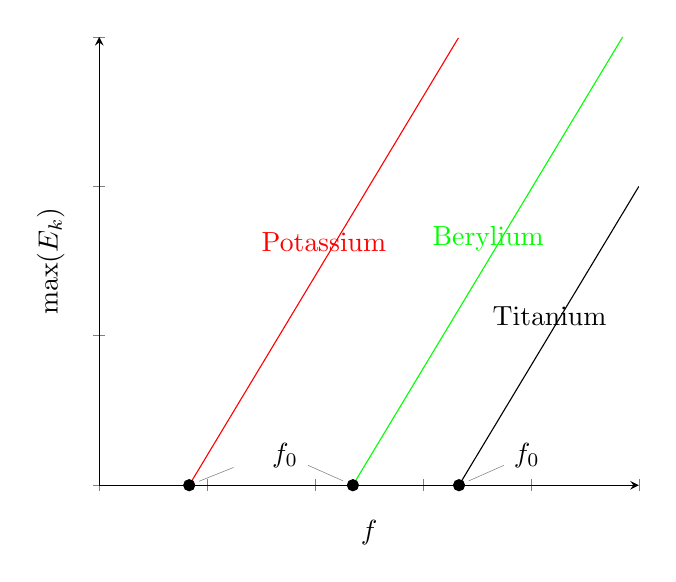
\begin{tikzpicture}
        \begin{axis}[
            axis lines = left,
            xlabel = $f$,
            ylabel = $\max(E_k)$,
            domain=0:10,
            xmin=0, xmax=10, ymin=0, ymax=15,
            yticklabels=\empty,
            xticklabels=\empty,
            samples=300,
        ]
        \addplot[color=red, restrict y to domain=0:15]   {3 * x - 5} node[anchor=east,above,pos=0.5] {\text{Potassium}};
        \addplot[color=green, restrict y to domain=0:15] {3 * x - 14.1} node[anchor=east,above,pos=0.5] {\text{Berylium}};
        \addplot[color=black, restrict y to domain=0:15] {3 * x - 20} node[anchor=east,above,pos=0.5] {\text{Titanium}};
        \addplot[mark=*] coordinates {(5/3,0)} node[pin=15:{}]{};
        \addplot[mark=*] coordinates {(4.7,0)} node[pin=170:{$f_0$}]{};
        \addplot[mark=*] coordinates {(20/3,0)} node[pin=10:{$f_0$}]{};
    \end{axis}
    \end{tikzpicture}
\end{figure}
\FloatBarrier

\begin{definition}{(\textbf{Threshold frequency})}
\textit{The threshold frequency $f_0$ of a photoemissive material is defined as the minimum frequency of the incident radiation which causes photoelectron emissions from the photoemissive surface.}
\end{definition}

Different materials have different threshold frequencies, however most elements (specifically metals) have threshold frequencies in the ultraviolet region of the electromagnetic spectrum.

\begin{definition}{(\textbf{The work function})}
\textit{The work function $\phi$ of a photoemissive material is defined as the minimum energy of the incident photons which causes photoelectron emission from the photoemissive surface.}
\end{definition}

Einstein described these factors using mathematics and the relationship between the maximum kinetic energy $\max(E_k)$ of the photoelectrons and the frequency of the absorbed photons $f$ and the threshold frequency $f_0$ of the photoemissive surface. 
\begin{equation}
    \max(E_k) = h(f - f_0)
\end{equation}
or if you prefer, to the energy of the absorbed photons $E$ and the \textbf{work function} of the surface
\begin{equation}
    \max(E_k) = E - \phi
\end{equation}
where the first term is the energy of the absorbed photons $E$ with frequency $f$ or wavelength $\lambda$ is
\begin{equation*}
    E = hf = \frac{h c}{\lambda}
\end{equation*}
where $c$ denotes the speed of light, and the second term is the \textbf{work function} $\phi$ which is defined as minimum energy required to free a single electron from the surface of the photoemissive surface and is expressed in terms of the threshold frequency $f_0$ of said surface or the threshold wavelength $\lambda_0$
\begin{equation}
    \phi = hf_0 = \frac{hc}{\lambda_0}
\end{equation}

So why did Einstein consider the maximum kinetic energy of the photoelectrons? Some electrons in the surface photoemissive material are closer to positive (metal) ions than others. Their relative positions affect how much energy is required to free them.  The work function is the minimum energy required to free an electron from the photoemissive surface (most electrons require a little more energy than the work function to free them). It follows from the conservation of energy that the electrons that requires the minimum amount of energy for photoemission to occur would have the most energy left from the incident photon. Only a few of the emitted photoelectrons have this \textit{maximum} kinetic energy - which is a fixed value based on the photoemissive material. 

Einstein also noticed a one-to-one interaction between photons and photoelectrons, that is a single incident photon on a photoemissive material with a frequency greater or equal to the threshold frequency of a photoemissive surface will cause a single photoelectron to be emitted. This interaction explains why an increase in intensity increases the rate of photoelectrons emitted. 

\subsection{Wave-particle duality}

The \textbf{wave-particle duality} is a model used to describe how all matter has both wave and particle properties. Electromagnetic radiation is a transverse wave, yet it is also a stream of particles (photons) so it has both wave and particle properties. Louis de Broglie realized that all matter travel through space as waves; matter is built from elementary particles (protons, neutrons, electrons, etc), however, matter is a probability wave (sometimes referred to as a matter wave or a de Broglie wave). 

We normally describe electrons as particles, they have a mass, a charge, can be accelerated, deflected by electric and magnetic fields; all properties we associate with particles. However, under certain conditions an electron can diffract and form a interference pattern in the same way as light. If we use an electron gun to fire an electron at a thin piece of polycrystalline graphite, which has carbon atoms arranged in different layers, the electrons pass between the individual carbon atoms in the graphite.  The gap between the atoms is so small that it is similar to the wavelength of the electrons and so the electrons diffract, as waves and form an interference pattern as seen in figures \ref{fig:electron-gun-electron-diffraction} and \ref{fig:electron-interference}.

\begin{figure}[h!]
    \centering
    \includegraphics[scale=0.1]{notes/images/Wave-Particle.JPG}
    \caption{Electron gun firing electrons at polycrystalline graphite}
    \label{fig:electron-gun-electron-diffraction}
\end{figure}
\FloatBarrier

\begin{figure}[h!]
    \centering
    \includegraphics{notes/images/Electron-Diffraction.JPG}
    \caption{Electron interference pattern}
    \label{fig:electron-interference}
\end{figure}
\FloatBarrier


In developing the wave-particle model, de Broglie combined the following equations to find the wavelength of a particle, 
\begin{equation}
    \vec{p} = m \vec{v} \hspace{1mm} \text{   and   } \hspace{1mm} \| \vec{p} \| = \frac{h}{\lambda} \hspace{0.3cm} \implies \hspace{0.3cm} \lambda = \frac{h}{\| \vec{p} \|} = \frac{h}{m \| \vec{v} \|},
\end{equation}
where $\lambda$ is the wavelength of the particle, $h$ is Planck's constant and $\vec{p}$ is the momentum of the particle. This is known as the \textbf{de Broglie equation}. We can also relate an object's kinetic energy $E_k$ to its wavelength by considering both the de Broglie equation and our general equation for kinetic energy. From the equation above, we have
\begin{equation}
    \lambda = \frac{h}{m \| \vec{v} \|}
\end{equation}
If we can find an expression for $m \| \vec{v} \|$ that includes $E_k$ we can determine the relationship between a particle's kinetic energy and its wavelength. Rearranging the follow relationship
\begin{equation*}
    E_k = \frac{1}{2} m \| \vec{v} \|^2
\end{equation*}
yields, 
\begin{equation}
    m \| \vec{v} \| = \sqrt{2mE_k}.
\end{equation}
We can then substitute this expression into the de Broglie equation, giving
\begin{equation*}
    \lambda = \frac{h}{m \| \vec{v} \|} = \frac{h}{\sqrt{2mE_k}}.
\end{equation*}
As $h$ and $m$ are constants (if we are only concerned with classical mechanics), we can see that the wavelength of a particle is inversely proportional to the square root of it's kinetic energy.
\begin{equation*}
    \lambda \propto \frac{1}{\sqrt{E_k}}.
\end{equation*}

So why don't cars have wavelengths? Do people diffract? The answer lies in the fact that as particles become larger their wave properties become harder to observe. Since
\begin{equation*}
    \lambda \propto \frac{1}{\| \vec{p} \|},
\end{equation*}
as the particle's mass increases, it's momentum increases, so it's wavelength is much smaller, and therefore much harder to observe.

\section{Particle Physics}

\subsection{Rutherford's Alpha-particle Scattering Experiment}

In 1897, English Physicist J.J Thompson discovered the existence of the electron and showed they were smaller than an atom, referred to as a \textit{sub-atomic} particle. Using his discovery, he developed ``plum - pudding'' model of the atom; suggesting that an atom contained negative electrons (the plums) embedded in a uniform sea of positive charge (the dough). 

However, in 1911, Ernest Rutherford and Geiger experimentally showed that the positive charge of the atom existed in a tiny nucleus about $10^{-14}$m in size, thus showing most the atom was empty space. In Rutherford's experiment, a narrow beam of alpha particles, all of the same kinetic energy, from a radioactive source were targeted at a thin piece of gold foil which was only a few atoms thick. The alpha particles were scattered by the foil and detected on a zinc sulfide screen mounted in front of a microscope. Each particle hitting this screen produced a ting flash. The microscope was moved around in order to count the number of alpha particles scattered through different values of the angle $\theta$ per minute.

\begin{figure}[h!]
    \centering
    \includegraphics{notes/images/Rutherford.JPG}
    \caption{Rutherford's Scattering}
\end{figure}
\FloatBarrier

Rutherford concluded the most of the alpha particles passed straight through the gold foil with very little scattering, suggesting that atoms are mainly made of empty space. Furthermore, very few of the alpha particles - about 1 in every 10000 - were deflected through angles greater than $\pi/2$, hence there must be a tiny positive charged called the \textbf{nucleus}. 

In order to be defected at angles greater than $\pi/2$, the scattered alpha particle will momentarily stop a short distance $r$ from the nucleus, before being repelled. Applying the principle of the conservation of energy, we find that
\begin{equation}
    \text{Initial kinetic energy of alpha particle} = \text{Electrical potential energy at distance } r.
\end{equation}
So in this case, we have
\begin{equation}
    \frac{1}{2} m_{\alpha} \| \vec{v} \|^2 = k_e \frac{Q_{gold} Q_{\alpha}}{r}
\end{equation}
Solving for $r$, produces an \textit{upper limit} for the radius of the gold nucleus. More energetic alpha particles might get closer. 

\subsection{The Atom}

We now know that an atom consists of a \textbf{nucleus} containing \textbf{protons} (positively charged particles) and \textbf{neutrons} (particles with a net charge of zero) surrounded by \textit{shells} of \textbf{electrons}. The size of an atom is approximately $10^{-10}$, whereas the size of the nucleus is approximately $10^{-14}$, that is to say the size of an atom is $10000$ times larger than it's nucleus.  

As mentioned previously, the nucleus contains protons and neutrons, which have approximately the same mass. The term \textbf{nucleon} is used to refer to either a proton or a neutron. A proton has the charge of $+e$, where $e$ is the elementary charge. So a neutral atom has the same number of electrons and protons to produce a net charge of zero.

The nucleus of an atom for a particle element is represent as 
\begin{equation}
    _{Z}^A X,
\end{equation}
where $X$ is the chemical symbol of the element, $A$ is the nucleon number (the total number of protons and neutrons) and $Z$ is the proton number (also known as the atomic number). The number of neutrons $N$ in the nucleus is thus $N = A - Z$

\subsubsection*{Isotopes}

\textbf{Isotopes} are nuclei of the same element that have the same number of protons but different numbers of neutrons. All isotopes of an element undergo the same chemical reactions

\subsubsection*{Atomic mass}

The masses of atoms and nuclear particles are often expressed in \textbf{atomic mass units} ($u$). One atomic mass unit $1 u$ is one-twelfth the mass of a neutral carbon-12 atom. 

\subsubsection*{Nuclear Size and Density}

The radius of the nucleus naturally depends on the nucleon number $A$. Recall that fast moving electrons have a de Broglie wavelength about $10^{-15}$. Diffraction of such electrons have be used to empirically prove that the radius $R$ of a nucleus is given by 
\begin{equation}
    R = r_0 A^{1/3},
\end{equation}
where $A$ is the nucleon number and $r_0$ has the approximate value of $1.2$ $fm$ ($1$ $fm = 10^{-15}m$). We now assume that a nucleus is spherical in nature, and therefore it's volume is given by 
\begin{equation}
    V = \frac{4}{3} \pi r_0^3 A
\end{equation}
From the definition of atomic, the mass of any given nucleus is $m = Au$, hence the density of a nucleus is 
\begin{align}
    \rho &= \frac{Au}{\frac{4}{3} \pi r_0^3 A} \\
    &= \frac{3u}{4\pi r_0^3}
\end{align}
Hence the density of any atom is constant.

\subsubsection*{Nuclear Forces}

But if a Nucleus only contains protons and neutrons, what force is overcoming the repulsive electrostatics forces between the protons? The gravitational force between protons is too weak to overcome this force. Therefore there must be another force of attraction, that only acts within the nucleus, known as the \textbf{Strong Nuclear Force}.

This force binds the nucleons together within the nucleus. It acts over a very short range of approximately $10^{-15}$ m. The strong force overcomes the electrostatic repulsion at short range, but becomes repulsive over a long range. 


\begin{figure}[h!]
    \centering
    \includegraphics{notes/images/StrongNuclear5.JPG}
    \caption{Strong Nuclear Force between two neutrons (or a neutron and a proton)}
\end{figure}
\FloatBarrier

\begin{figure}[h!]
    \centering
    \includegraphics{notes/images/StrongNuclear4.JPG}
    \caption{Strong Nuclear Force between two protons}
\end{figure}
\FloatBarrier

The graphs above show that the force is independent of charge and only acts over a range of approximately of 5 fm. The force is powerfully attractive between nucleons at distances of about 1 fm between their centers, but rapidly decreases to insignificance at distances beyond about 3 fm (for neutron and proton interaction) and 4 fm (for proton and proton interaction). At very short distances less than 0.5 fm, it becomes repulsive, and is responsible for the physical size of nuclei, since the nucleons can come no closer than the force allows. Thus preventing the nucleus from collapsing.

\subsection{Antiparticles}
\label{subsection:antiparticles}

In 1928, Paul Dirac invents the relativistic Schodinger equation, known as the Dirac equation. When applied to an electron, the wave equation refers to both an electron with charge $e$ (a positron) and an electron with charge $-e$. From this Dirac predicted that every particle has a corresponding \textbf{antiparticle} which has the same mass, opposite charge and opposite spin. For example, the antiparticle of an electron $e^{-}$ is the positron $e^{+}$. The table below lists some common particles are their corresponding antiparticle;

\begin{table}[h!]
    \centering
    \begin{tabular}{c|c}
        \textit{Particle} & \textit{Antiparticle} \\
        \hline
        \text{proton} $p$ & \text{antiproton} $\overline{p}$ \\
        \text{neutron} $n$ & \text{antineutron} $\overline{n}$ \\
        \text{electron} $e^{-}$ & \text{positron} $e^{+}$ \\
        \text{up quark} $u$ & \text{anti up quark} $\overline{u}$ \\
        \text{down quark} $d$ & \text{anti down quark} $\overline{d}$ \\
        \text{strange quark} $s$ & \text{anti strange quark} $\overline{s}$ \\
        \text{neutrino} $v$ & \text{anti neutrino} $\overline{v}$ \\
    \end{tabular}
\end{table}
\FloatBarrier

Dirac also theorised that if a particle meets it's antiparticle they \textbf{annihilate} where the masses of both particle and antiparticle are converted into a high-energy pair of photons. For example,
\begin{equation}
    e^- + e^+ \longrightarrow 2 \gamma
\end{equation}
In order to conserve momentum, the 2 photons will travel in opposite directions. 

\begin{figure}[h!]
    \centering
    \includegraphics[scale=0.15]{notes/images/Annihilation.JPG}
    \caption{Electron and Positron annihilation}
\end{figure}
\FloatBarrier

\textbf{Pair production} is the opposite process to annihilation, where high energy photons create a particle-antiparticle pair. 

\subsection{Quarks}

In 1963, American physicist Murrary Gell-Mann performed the deep inelastic scattering experiment. Gell-Mann postulated that nucleons contained particles called \textbf{Quarks}. In order to discover the structure of nucleons, electrons were fired at them in a similar experiment to Rutherford's alpha-particle scattering experiment. The results showed the existence of three concentrations of mass and charge within the nucleon, implying that a nucleon consisted of three quarks. 

The standard model of elementary particles requires six quarks and six anti-quarks. The six quarks are up, down, charm, strange, top and bottom denoted by $u, d, c, s, t$ and $b$, respectively. All quarks have a charge that is a fraction of the elementary charge $e$ (the only case where charge isn't quantized).

All the quarks are listed in the table below, but for A2 Physics we only need to use up, down and strange quarks and their anti-quarks. 

\begin{table}[h!]
    \centering
    \begin{tabular}{c | c c c c}
        \textit{Quark} & \textit{Symbol} & \textit{Relative Charge*} & \textit{Baryon Number} & \textit{Strangeness}\\
        \hline
        \text{up} & $u$ & $+\frac{2}{3}$ & $\frac{1}{3}$ & $0$ \\[2mm]
        \text{down} & $d$ & $-\frac{1}{3}$ & $\frac{1}{3}$ & $0$\\[2mm]
        \text{charm} & $c$ & $+\frac{2}{3}$ & $\frac{1}{3}$ & $0$ \\[2mm]
        \text{strange} & $s$ & $-\frac{1}{3}$ & $\frac{1}{3}$ & $-1$\\[2mm]
        \text{top} & $t$ & $+\frac{2}{3}$ & $\frac{1}{3}$ & $0$ \\[2mm]
        \text{bottom} & $b$ & $-\frac{1}{3}$ & $\frac{1}{3}$ & $0$
    \end{tabular}
\end{table}
\FloatBarrier

\begin{table}[h!]
    \centering
    \begin{tabular}{c | c c c c}
        \textit{Anti-quark} & \textit{Symbol} & \textit{Relative Charge*} & \textit{Baryon Number} & \textit{Strangeness}\\
        \hline
        \text{anti up} & $\overline{u}$ & $-\frac{2}{3}$ & $-\frac{1}{3}$ & $0$ \\[2mm]
        \text{anti down} & $\overline{d}$ & $+\frac{1}{3}$ & $-\frac{1}{3}$ & $0$\\[2mm]
        \text{anti charm} & $\overline{c}$ & $-\frac{2}{3}$ & $-\frac{1}{3}$ & $0$ \\[2mm]
        \text{anti strange} & $\overline{s}$ & $+\frac{1}{3}$ & $-\frac{1}{3}$ & $1$\\[2mm]
        \text{anti top} & $\overline{t}$ & $-\frac{2}{3}$ & $-\frac{1}{3}$ & $0$ \\[2mm]
        \text{anti bottom} & $\overline{b}$ & $+\frac{1}{3}$ & $-\frac{1}{3}$ & $0$
    \end{tabular}
\end{table}
\FloatBarrier

\noindent * relative to the elementary charge. 

\subsubsection*{Strangeness}

If a particle contains a strange quark it is said to be a \textbf{strange} particle. Strange particles are unusually long lived. The ``strangeness'' value of a particle lies in the range $[-3, 3]$. In all interactions containing strong nuclear force, strangeness is conserved. However, in weak interactions, the strangeness value may change by $-1, 0$ or $+1$. 

\subsection{Fundamental and Non-Fundamental Particles}

\noindent All particles are split into two families - fundamental particles and non-fundamental particles. 
\begin{itemize}
    \item \textbf{Fundamental Particles}: Particles with no internal structure that cannot be broken down into smaller constituents. Examples include Quarks (see above), Leptons and Exchange particles:
    \begin{itemize}
        \item \textbf{Leptons}: Leptons are particles and antiparticles that are not affected by the strong nuclear forces. Examples include electrons, muons, taus and neutrinos. All leptons have a lepton number of $1$ and all anti-leptons have a lepton number of $-1$. In all particle interactions, the lepton number must be conserved.  
        \item \textbf{Exchange particles}: Exchange particles are virtual particles that mediate the interaction between two other particles. Examples include gluons and photons. 
    \end{itemize}
    \item \textbf{Non-Fundamental Particles}: In A2 Physics, all non-fundamental particles are \textbf{Hadrons} which are made from quarks. \textbf{Hadrons} are particles and antiparticles that are affected by strong nuclear forces. Examples include protons, neutrons (baryons), pions and kaons (mesons)
    \begin{itemize}
        \item \textbf{Baryons}: Baryons are particles and antiparticle consisting of \textbf{three quarks}. Protons and neutrons are baryons, with the following quark compositions 
        \begin{equation*}
            p = uud \text{ and } n = udd.
        \end{equation*}
        Anti-protons and anti-neutrons are anti-baryons with the following quark compositions
        \begin{equation*}
            \overline{p} = \overline{u}\overline{u}\overline{d} \text{ and } \overline{n} = \overline{u}\overline{d}\overline{d}.
        \end{equation*}
        All baryons have a baryon number of $1$ and all anti-baryons have a baryon number of $-1$. In all particle interactions, the baryon number must be conserved.
        \item \textbf{Mesons}: Mesons are particles and antiparticles consisting of a quark and a anti-quark pair. For example, the meson known as a pion denoted by $\pi^0, \pi^+$ has the following quark composition:
        \begin{equation*}
            \pi^0 = u \overline{u} \text{ or } \pi^0 = d \overline{d} \text{ and } \pi^+ = u \overline{d}  
        \end{equation*}
        The anti-pion (an anti-meson) is $\pi^0$ and $\pi^-$, so 
        \begin{equation*}
            \overline{\pi^0} = \pi^0 \text{ and } \overline{\pi^+} = \pi^- = \overline{u} d
        \end{equation*}
        The Kaon $K$ is meson and a strange particle (with a strangeness of $1$), with the following quark composition
        \begin{equation*}
            K^0 = d \overline{s} \text{ and } K^+ = u \overline{s}
        \end{equation*}
        The anti-kaon is an anti-meson with a strangeness of $-1$ with the following compositions
        \begin{equation*}
            \overline{K^0} = K^0 \text{ and } \overline{K^+} + K^- = \overline{u} s.
        \end{equation*}
    \end{itemize}
\end{itemize}

\noindent Note that in all particle interactions, four quantities are conserved:
\begin{itemize}
    \item Charge
    \item Baryon Number
    \item Lepton Number
    \item Strangeness 
\end{itemize}

\subsection{Beta Decay}

There are various types of radiation that unstable nuclei emit, such as $\alpha$, $\beta$ and $\gamma$. We will discuss these types of radiations in more detail in section ??.

Beta decays is the emission of either electrons $\beta^-$ decay, or positrons $\beta^+$ decay. These emissions must be related to changes taking place within the nuclei of the atoms. In the case of beta day, the changes occur to the neutrons or the protons. The force responsible for beta decay is the \textbf{weak nuclear force}. The weak nuclear force acts between quarks in the nucleus and leptons. The weak force has a very short range, approximately $10^{-18}$ m.

In $\beta^-$ decay, a neutron $_0^1 n$ in an unstable nucleus decays into a proton $_1^1 p$, an electron $_{-1}^0 e$ and an electron anti-neutrino $\overline{v_e}$. 
\begin{equation}
    _0^1 n \longrightarrow \hspace{1mm} _1^1 p + _{-1}^{0} e + _0^0 \overline{v_e} + \text{energy}
\end{equation}


In $\beta^+$ decay, a proton $_1^1 p$ in an unstable nucleus decays into a neutron $_0^1 n$, a positron $_{1}^0 e$ and an electron neutrino $v_e$. 
\begin{equation}
    _1^1 p \longrightarrow \hspace{1mm} _0^1 n + _{1}^{0} e + _0^0 v_e + \text{energy}
\end{equation}

Since protons and neutrons consist of quarks; each type of beta decay is associated with the decay of a specific quark within the proton or the neutron. In $\beta^-$ decay one of the down quarks changes \textbf{flavour} to an up quark, so the decay equation is
\begin{equation}
    d \longrightarrow \hspace{1mm} u + _{-1}^{0} e + _0^0 \overline{v_e} + \text{energy}
\end{equation}

Similarly, in $\beta^+$ decay, one of the up quarks changes \textbf{flavour} to a down quark, hence 

\begin{equation}
    u \longrightarrow \hspace{1mm} d + _{1}^{0} e + _0^0 v_e + \text{energy}
\end{equation}

\section{Nuclear Physics}

\subsection{Radioactive Decay}

Radioactive decay is a process whereby a nucleus attempts to stabilise itself by releasing energy through radiation. A negligible amount can be detected in nature, and this is called \textbf{background radiation}, a large proportion of which is radon gas resultant from the decay of uranium within rocks. \textbf{Activity} is the measure of rate of radioactive decay, with unit \textbf{Becquerel}. 

Say \(N\) is the number of undecayed nuclei in a sample. While \(N\) is obviously discrete, being a natural number, it is often large enough to be well-approximated as a continuous variable. While, it is a random process, it is impossible to predict when any undecayed nuclei may decay, (and if we are to treat \(N\) as continuous variable, the probability of decay in any particular instant is zero) we can suppose it is equally likely that undecayed nuclei will decay in one instant than any other. 

As \(N\) is a continuous quantity dependent on \(t\), it makes sense to take a derivative in the usual sense. 

\begin{definition}{(\textbf{Activity})}
\textit{We define the activity of a sample at time \(t_0\) as:}

\begin{equation}
A(t = t_0) = \left. \frac{\mathop{\mathrm{d} N}}{\mathop{\mathrm{d} t}} \right|_{t = t_0}
\end{equation}
\end{definition} 

We know that the likelihood of decay at any given time will be proportional to the number of remaining undecayed nuclei at that instant, since we supposed that each have an equal probability of decaying in that instant. We can therefore write 
\begin{equation}
A \propto N
\end{equation}

As the activity of the sample will decrease with time, we expect the constant of proportionality here to be negative. Write this constant of proportionality \(-\lambda\), and we call \(\lambda\) the \textbf{decay constant}. Then we have the following differential equation 
\begin{equation}
\frac{\mathop{\mathrm{d} N}}{\mathop{\mathrm{d} t}} = -\lambda N.
\end{equation} 
If the initial number of undecayed nuclei is \(N_0\), we should require that \(N = N_0\) at \(t=0\).  Which can trivially be solved by the separation of variables: 
\begin{align} 
\frac 1 N \frac{\mathop{\mathrm{d} N}}{\mathop{\mathrm{d} t}} &= -\lambda \\ 
\int_{N_0}^N \frac {\mathop{\mathrm{d} N}} N &= -\lambda \int_0^t \mathop{\mathrm{d} t} \\ 
\ln \left | \frac{N}{N_0} \right| &= -\lambda t 
\\ N &= N_0 \exp(-\lambda t)
\end{align}
Hence, activity can then be determined by taking the derivative of the $N$ 
\begin{equation} 
A = \frac{\mathop{\mathrm{d} N}}{\mathop{\mathrm{d} t}} = -\lambda N_0 \exp(-\lambda t)
\end{equation} 

As we have defined the activity of the sample as being \(-\lambda N\) at any instant, the initial activity of the sample \(A_0\) is equal to \(-\lambda N_0\) where \(N_0\) is the initial number of undecayed nuclei. With that we may rewrite the original equation as 
\begin{equation} 
A = A_0 \exp(-\lambda t)
\end{equation} 

We may be interested in ways to calculate the decay constant. A common measure of the radioactivity of a substance is its half-life: 

\begin{definition}{(\textbf{Half-Life})}
\textit{The \textbf{half-life} of a particular the sample is the length of time it takes for half of the unstable nuclei in the sample to decay.}
\end{definition} 

We can determine this using, for example, the graph of the activity of the sample against time (which we could produce electronically with aid of a GM counter). We can then use this to then determine the decay constant \(\lambda\). Let use denote the half-life of a particular sample as \(t_{1/2}\), and its initial undecayed nuclei count as \(N_0\). At \(t_{1/2}\), the count of undecayed nuclei is \(\frac 1 2 N_0\), so
\begin{equation} 
\frac{N_0} 2 = N_0 e^{-\lambda t_{1/2}}
\end{equation} 
Dividing through by \(N_0\) and taking the natural log of both sides
\begin{equation*}
\ln \frac 1 2 = -\lambda t_{1/2}
\end{equation*} 
writing \(\ln \frac 1 2 = -\ln 2\), we have
\begin{equation} 
\lambda = \frac {\ln 2} {t_{1/2}}.
\end{equation} 

\subsection{Radioactive decay processes}
We have spoke a lot about the rate at which nuclei decay, but we have not yet discussed the processes by which they decay. 

\textbf{\(\alpha\) decay} occurs when a nuclei has too many protons compared to the number of neutrons. This causes the nucleus to eject a helium-4 atom, comprised of 2 protons and 2 neutrons as to reduce the ratio between protons and neutrons. This type of radiation can pose significant danger, as it is strongly ionising and can therefore cause serious damage if put into contact with, for example, internal organs. (if an alpha admitter is accidentally consumed) However, as it is so ionising, it quickly loses kinetic energy and can therefore be easily absorbed. It is absorbed by a few centimetres of air or a sheet of paper. An example of an \(\alpha\) decay process is: 

\begin{equation*} 
_{95}^{241} \textrm{Am} \longrightarrow \hspace{1mm} _{93}^{237} \textrm{Np} + _2^4 \alpha
\end{equation*} 

\textbf{\(\beta^-\) decay} occurs when there a nuclei has too many neutrons compared to the number of protons. This causes a neutron to decay into a proton (by changing its quark configuration) and an electron, (which we call a \(\beta\) particle) which is ejected along with an antineutrino. The \(\beta\) particle has half the charge of an \(\alpha\) particle and is much smaller, so is less ionising. But with this, it loses kinetic energy at a slower rate, and so can penetrate further. A thin sheet of aluminium is usually sufficient to absorb a \(\beta\) particle. 

\begin{equation*} 
_{6}^{14} \textrm{C} \longrightarrow \hspace{1mm} _{7}^{14} \textrm{N} + _{-1}^{0} \beta + _{0}^{0} \overline{v}
\end{equation*} 

\textbf{Gamma decay} occurs when a massive nuclei has too much energy, usually occurring immediately after \(\alpha\) or \(\beta\) decay as the nucleus is left in an excited state. Unlike the other types of decay, this does not release any particles and hence does not change the nuclei in any way. Instead, gamma rays are high frequency electromagnetic waves. As they are EM waves and not particles, they do not have mass or charge, so will rarely interact. However, this means that they are extremely difficult to absorb, and can only be absorbed by several inches of lead or several metres of concrete. This means that gamma is most often considered the most dangerous radiation.  

\subsection{Relativity and Einstein's Mass-Energy Equation}

Let us consider momentum in both Classical and Relativistic mechanics. In both models, momentum is defined as 
\begin{equation}
    \vec{p} = m \vec{v},
\end{equation}
and momentum is conserved in a closed system, that is 
\begin{equation}
    \frac{\mathop{\mathrm{d}}}{\mathop{\mathrm{d}t}} \sum \vec{p} = 0
\end{equation}
However, in a classical model we have
\begin{equation}
    \lim_{\vec{v} \rightarrow \infty} \vec{p} = \infty    
\end{equation} 
This is not allowed in special relativity, hence we redefine mass so it has a velocity dependence, 
\begin{equation}
    m = m_0 f(v).
\end{equation}
such that $f(v = 0) = 1$. In fact
\begin{equation}
    m = m_0 \gamma = \frac{m_0}{\sqrt{1 - v^2 / c^2}},
\end{equation}
where $c$ is the speed of light in a vacuum. So we have
\begin{equation}
    \vec{p} = \frac{m_0 \vec{v}}{\sqrt{1 - v^2 / c^2}},
\end{equation}
where $m_0$ is the \textbf{rest mass}. So in a relativistic model, Newton's second law of motion for a single particle of rest mass $m_0$ becomes
\begin{align}
    \vec{F} &= \frac{\mathop{\mathrm{d}\vec{p}}}{\mathop{\mathrm{d}t}} \\
    &= m_0 \frac{\mathrm{d}}{\mathop{\mathrm{d}t}} \gamma \vec{v} \\
    &= m_0 \left(\gamma \vec{a} + \vec{v} \frac{\mathop{\mathrm{d}\gamma}}{\mathop{\mathrm{d}t}}\right)
\end{align}
We will now consider the relativistic kinetic energy of the particle, by considering the work done by $\vec{F}$. So by definition, we have
\begin{equation}
    W = \int_C \vec{F} \cdot \mathop{\mathrm{d}\vec{r}}
    \label{eq:sr-work-1}
\end{equation}
To simplify the model, we will consider motion in one-dimension, allowing us to replace the line integral with a regular integral. Also, note that $\mathop{\mathrm{d}\vec{r}} = \vec{v} \mathop{\mathrm{d}t}$. Applying this to equation \ref{eq:sr-work-1} gives us
\begin{equation}
    W = \int_0^t m_0 v \left(\gamma \frac{\mathop{\mathrm{d}v}}{\mathop{\mathrm{d}t}} + v \frac{\mathop{\mathrm{d}\gamma}}{\mathop{\mathrm{d}t}}\right) \mathop{\mathrm{d}t}.
    \label{eq:sr-work-2}
\end{equation}
Let us now consider the time derivative of gamma, 
\begin{align}
    \frac{\mathop{\mathrm{d}\gamma}}{\mathop{\mathrm{d}t}} &= \frac{\mathrm{d}}{\mathop{\mathrm{d}t}} \frac{1}{\sqrt{1 - v^2/c^2}} \\
    &= - \frac{1}{2} (1 - v^2 / c^2)^{-\frac{3}{2}} \left(-\frac{2v}{c^2} \frac{\mathop{\mathrm{d}v}}{\mathop{\mathrm{d}t}}\right) \\
    &= v \frac{\gamma^3 }{c^2} \frac{\mathop{\mathrm{d}v}}{\mathop{\mathrm{d}t}} \label{eq:sr-dgamma-1}
\end{align}
Substituting the above expression into equation \ref{eq:sr-work-2} gives
\begin{align}
    W &= \int_0^t m_0 v \left(\gamma \frac{\mathop{\mathrm{d}v}}{\mathop{\mathrm{d}t}} + \gamma^3 \frac{v^2}{c^2} \frac{\mathop{\mathrm{d}v}}{\mathop{\mathrm{d}t}}\right) \mathop{\mathrm{d}t} \\
    &= \int_0^t m_0 v \gamma \frac{\mathop{\mathrm{d}v}}{\mathop{\mathrm{d}t}} \left(1 + \frac{v^2}{c^2} \gamma^2\right) \mathop{\mathrm{d}t}
\end{align}
Considering the 5$^{th}$ term of the integrand above gives
\begin{align}
    1 + \frac{v^2}{c^2} \gamma^2 &= 1 + \frac{v^2}{c^2} \frac{1}{1-v^2/c^2} \\
    &= \frac{1-v^2/c^2+v^2/c^2}{1-v^2/c^2} \\ 
    &= \gamma^2
\end{align}
Hence the work done is 
\begin{equation}
    W = \int_0^t m_0 v \gamma^3 \frac{\mathop{\mathrm{d}v}}{\mathop{\mathrm{d}t}} \mathop{\mathrm{d}t}. 
\end{equation}
Rearranging equation \ref{eq:sr-dgamma-1} yields
\begin{equation}
    c^2 \frac{\mathop{\mathrm{d}\gamma}}{\mathop{\mathrm{d}t}} = v \gamma^3 \frac{\mathop{\mathrm{d}v}}{\mathop{\mathrm{d}t}}
\end{equation}
Applying this to the expression for work done above, we find that 
\begin{align}
    W = \int_0^t m_0 c^2 \frac{\mathop{\mathrm{d}\gamma}}{\mathop{\mathrm{d}t}} \mathop{\mathrm{d}t} 
\end{align}
Suppose the particle we're considering is at rest at time $t = 0$, so we have
\begin{align}
    W &= m_0 c^2 \int_1^\gamma \mathop{\mathrm{d}\gamma} \\
    &= m_0 c^2 (\gamma - 1)
\end{align}
This is the expression for \textbf{Relativistic kinetic energy} $E_{k,r}$. It follows that for small $v^2/c^2$, we have
\begin{equation}
    \sqrt{1 - \frac{v^2}{c^2}} \approx 1 - \frac{1}{2}\frac{v^2}{c^2}.
\end{equation}
So 
\begin{align}
    E_{k,r} &= m_0 c^2 \left(\frac{1}{1-v^2/2c^2} - 1\right) \\
    &= m_0 c^2 \frac{v^2}{2c^2} \\
    &= \frac{1}{2} m_0 v^2
\end{align}
The classical equation for kinetic energy!. Now let us define the energy $E$ of the particle as 
\begin{equation}
    E = E_{k,r} + m_0 c^2 = \gamma m_0 c^2.
\end{equation}
Now consider $E^2 - (pc^2)$, where $p$ is the momentum of the particle (in our one-dimension model). So we have
\begin{align}
    E^2 - (pc)^2 &= m_0^2 c^4 \gamma^2 - \gamma^2 m_0^2 c^2 v^2 \\
    &= (m_0c)^2 \gamma^2 (c^2 - v^2).
\end{align}
However, recall that
\begin{equation}
    \gamma^2 = \frac{1}{1-v^2/c^2} = \frac{c^2}{c^2 - v^2},
\end{equation}
then
\begin{equation}
    E^2 - (pc)^2 = (m_0c^2)^2
\end{equation}
Now when the particle is at rest, i.e $v = 0$, we have
\begin{equation}
    E = m_0 c^2.
\end{equation}
Einstein's mass-energy equation! The interpretations of this equation are
\begin{itemize}
    \item Firstly, mass is a form of energy. The interaction of a particle and it's anti particle, known as \textbf{annihilation}, is an example of this (see section \ref{subsection:antiparticles}).
    \item Alternatively, we could say energy has mass. This is similarly demonstrated by \textbf{pair production} (see section \ref{subsection:antiparticles})
\end{itemize}  

\subsection{Einstein's mass-energy equation and Binding energy}
\begin{definition}{(\textbf{Atomic mass unit})} 
\textit{We define \(u\) to be \(\frac 1 {12}\)th of the mass of a carbon-12 atom. \(u \approx 1.67 \times 10^{-27} \textrm{kg}\) to 3 s.f.}
\end{definition} 

The mass of a nucleon is then about \(1u\). While we would expect the mass of a nucleus to be given by the sum of the masses of its constituent nucleons, this is not the case. The measured mass will always be less than this. The difference between these two masses is the \textbf{mass deficit}. This deficit is caused because a small amount of the mass is converted to \textbf{binding energy} - which is needed to hold the nucleus together. 

\begin{definition}{(\textbf{Binding energy})}
\textit{We define the binding energy $E_b$ of a nucleus as the minimum energy required to completely separate a nucleus into its constituent nucleons.}
\end{definition}
\begin{definition}({\textbf{Mass deficit}})
\textit{We define the mass deficit $\Delta m$ as the difference between the mass of the completely separated nucleons and the mass of the nucleus.}
\end{definition}

The binding energy $E_b$ can be calculated using Einstein's mass-energy equation: 
\begin{equation*}
E_b = c^2 \Delta m
\end{equation*} 

where \(E_b\) is the required binding energy, \(c\) is the speed of light in a vacuum and \(\Delta m\) is the mass deficit. Due to the comparatively low mass of electrons compared to the other nucleons, they are often ignored in calculations of mass. 

\begin{example}
For example, take a carbon-\(12\) atom, which has 6 protons (with mass \(\approx 1.008665u\)) and 6 neutrons (with mass \(\approx 1.007276u\)). From the definition of \(u\), this atom has mass \(12u\), so the mass deficit is approximately \((12 - 6 \cdot 1.008665 - 6 \cdot 1.007276)u = - 0.098937u\), giving a binding energy of approximately \(92.3 \textrm{MeV}\). 
\end{example}
\begin{example}
Consider a uranium-$235$ atom, which has $92$ protons and $143$ neutrons. Therefore the mass of the nucleons are $(92 \times 1.007276u) + (143 \times 1.008665u) = 236.908487u$. Given the mass of the nucleus is $235.004393u$, then the mass deficit is 
\begin{align}
    \Delta m &= (235.004393 - 236.908487)u = - 1.904094 u\\ 
    &= - 1.904094 \times 1.661 \times 10^{-27}\\ 
    &= - 3.162700 \times 10^{-27} \text{ kg}.
\end{align}
So the binding energy of the nucleus is 
\begin{align}
    E_b &= 3.162700 \times 10^{-27} \times (3 \times 10^8)^2 \\
    &= 2.846430 \times 10^{-10} \text{ J} \\
    &= 1779 \text{ MeV}.
\end{align}
\end{example}

We may be interested in how much energy it takes to remove a nucleon from an atom. If more energy is required to remove a nucleon from the nucleus, we can conclude that the nucleus is more "tightly bound" and hence harder (ie. requires more energy) to break apart. To quantify this we take the \textbf{binding energy per nucleon}, by dividing the mass by the number of nucleons. (we are merely taking an average, so the difference in mass between protons and neutrons does not matter.)  

\begin{figure}[h!]
    \centering
    \includegraphics[scale=0.75]{notes/images/BE-Per-Nucleon.JPG}
    \caption{Binding energy per nucleon against nucleon number $A$ for nuclei}
    \label{fig:be-per-nucleon}
\end{figure}
\FloatBarrier

The figure above shows the binding energy per nucleon against nucleon number $A$. Some deductions can be made about radioactive decay, nuclear fission and fusion from the graph;
\begin{itemize}
    \item For nuclei with $A < 56$, the binding energy per nucleon increases as $A$ increases.
    \item For nuclei with $A > 56$, the binding energy per nucleon decreases as $A$ increases.
    \item $_{26}^{56}$Fe has the greatest binding energy per nucleon and is the most stable isotope in nature.
    \item $_{2}^4$He nuclei has an abnormally greater binding energy per nucleon than it's neighbours. $_6^{12}$C and $_8^{16}$O also exhibit this property.
    \item In radioactive decay, the graph shows the total binding energy of the parent nucleus is less than the binding energy of the daughter nucleus and the alpha particle. The extra energy is released as kinetic energy.
    \item In a nuclear fission reaction, a nucleus with a high $A$ splits into lower $A$ number nuclei. Energy is released because the two daughter nuclei have higher binding energies than the parent nucleus. 
    \item In a nuclear fusion reaction, two low $A$ number nuclei amalgamate to form a higher $A$ number nucleus, which has a much greater binding energy than the initial nuclei and therefore energy is released. 
    
\end{itemize}
\subsection{Fission}
Nuclear fission is the splitting of a heavy nucleus into lighter daughter nuclei. These lighter daughter nuclei have a greater binding energy per nucleon than that of the heavy nucleus, so the sum of the masses of the daughter nuclei is less than that of the larger nucleus. Due to mass-energy conservation, this releases energy equal to \(E = c^2 \Delta m\). 

The need for heavier nuclei can be seen in Figure \ref{fig:be-per-nucleon}, as beyond iron-56, the binding energy per nucleon decreases as nucleon number increases, so performing fission with nuclei sufficiently heavier than iron causes the desired effect.  

Uranium is the most common fuel used in nuclear fission. The uranium-235 isotope easily undergoes fission on absorbing a slow neutron, known as a \textbf{thermal neutron} (because their mean kinetic energy is similar to the thermal energy of the particles in the reactor core). A typical induced fission reaction of uranium-235 by a thermal neutron is
\begin{equation}
    _{92}^{235}\text{U} + _0^1\text{n} \longrightarrow \hspace{1mm} _{92}^{236}\text{U} \longrightarrow \hspace{1mm} _{56}^{141}\text{Ba} + _{36}^{92}\text{Kr} + 3 \hspace{1mm} _{0}^1\text{n}.
\end{equation}
The uranium-235 nucleus captures the neutron, becomes a highly unstable nucleus of uranium-236. The uranium-236 nucleus than splits, the daughter nuclei produced in the example above are barium-141 and krypton-92. Three fast neutrons are also produced. 

\subsubsection*{Chain Reactions}

If the three fast neutrons discussed above could be slowed, they could induce further fission reactions. This causes a \textbf{nuclear chain reaction}.

\begin{definition}{(\textbf{Nuclear Chain Reaction})}
\textit{A nuclear chain reaction is series of nuclear reactions, each initiated by the preceding nuclear reaction.}
\end{definition}

In a nuclear fission chain reaction, the \textbf{mean generation time} $\Lambda$ is the average time from a neutron emission to a capture that results in fission. 

\begin{equation}
    \Lambda = \frac{l}{k},
\end{equation}
where $l$ is the neutron life time and $k$ is the effective neutron multiplication factor, described below. 

The neutron multiplication factor $k$ is the average number of neutrons from one fission that induce another fission. We can consider how $k$ determines how a nuclear chain reaction proceeds. Firstly, we note that the following differential equation used to model a nuclear chain reaction (note that I am unsure about the validity of this relationship, as I derived it using a thought experiment).
\begin{equation}
    \frac{\mathop{\mathrm{d}N}}{\mathop{\mathrm{d}t}} = \frac{k-1}{\tau} N - \kappa N,
\end{equation}
where $\tau$ is the mean time for one cycle and $\kappa$ is to account for some inhibitors. If the initial number of neutrons is $N_0$. We can solve the differential equation by the separation of variables
\begin{align}
    \frac{1}{N} \frac{\mathop{\mathrm{d}N}}{\mathop{\mathrm{d}t}} &= \frac{k-1}{\tau} - \kappa \\
    \int_{N_0}^N \frac{\mathop{\mathrm{d}N}}{N} &= \left(\frac{k-1}{\tau} - \kappa\right) \int_0^t \mathop{\mathrm{d}t} \\
    \ln\left|\frac{N}{N_0}\right| &= \left(\frac{k-1}{\tau} - \kappa\right) t\\
    N &= N_0 \exp\left(\left[\frac{k-1}{\tau} - \kappa\right]t\right) 
\end{align}
\begin{example}
So for example, suppose we consider the number of neutrons in a reaction with an effective neutron multiplication factor of $k = 1.01$, a cycle time of $\tau = 0.001$s with no inhibitors (hence $\kappa = 0$) after one second has elapsed;
\begin{equation}
    \frac{N}{N_0} = e^{0.01/0.001} = e^{10}
\end{equation}
So it is clear that $k>1$, we have an exponential increase in neutrons.
\end{example}
\noindent So the value of $k$ determines how the nuclear reaction proceeds
\begin{itemize}
    \item $k<1$: \textbf{Subcriticality}: The system cannot sustain a chain reaction, and any beginning of a chain reaction dies out over time.
    \item $k = 1$: \textbf{Criticality}: Every fission causes an average of one more fission, leading to a fission level that is constant. This is optimal for a nuclear power plant (provided inhibitors are minimised).
    \item $k > 1$: \textbf{Supercriticality}: For every fission reaction, it is likely that there will be $k$ fissions after the next mean generation time. The number of fissions reactions increases exponentially, according to the equation
    \begin{equation}
        \text{number of reactions} = e^{(k-1)t/\Lambda},
    \end{equation}
    where $t$ is the elapsed time. 
\end{itemize}

\subsubsection*{Fission Reactors}

Firstly, we note that a uranium reactor will \textbf{never} explode even if it goes supercritical. As the reactor core heats up, the kinetic energy of the thermal neutrons increases, thus decreasing the number of fission reactions (as slow moving neutrons are required to induce a reaction). So the reaction stabilises at a high temperature, however this leads to a \textbf{MELTDOWN}. A meltdown is where the nuclear material in the reactor melts (\textit{pretty self explanatory really...}).

\begin{figure}[h!]
    \centering
    \includegraphics[scale=0.75]{notes/images/Reactor.JPG}
    \caption{Nuclear Reactor Design.}
\end{figure}
\FloatBarrier

In this course, we'll consider the a common fission reactor design, known as a \textbf{Thermal reactor} (see figure above). 
%a thermal reactor makes uses of delayed neutron emission by designing the reactor to be subcritical to prompt neutrons and use the delayed neutrons to take it to critical. So following a nuclear fission reaction, the fast prompt neutrons are removed. They are then thermalized (increase the thermal energy of the neutron) and allow them to drift back into the fuel. 
The \textbf{fuel rods} in a reactor are spaced evenly in a steel-concrete vessel known as the \textbf{core}. A \textbf{coolant} removes the thermal energy produced by the fission reactions. The fuel rods are surrounded by the \textbf{moderator}, and \textbf{control rods}. The \textit{fuel rods} consist of enriched uranium, mainly uranium-238 and a small amount of uranium-235. The \textit{moderator} slows down the neutrons produced by nuclear fission reactions. The mean kinetic energy of the thermal neutrons $\overline{E_k}$ is given by
\begin{equation}
    \overline{E_k} = \frac{3}{2}kT,
\end{equation}
where $T$ is the thermodynamic temperature of the core. When a fast moving neutron collides elastically with protons in water or with carbon nuclei, they transfer significant kinetic energy and slow down. Suggesting water and carbon are good moderators. Many reactors uses water as both a moderator and a coolant. The \textit{control rods} are designed to absorb the neutrons, most commonly boron or cadmium. The position of the control rods is adjusted to ensure that the reactor maintains criticality. 

Nuclear fission reactors produce extremely hazardous materials such as Plutonium-239. Radioactive waste from reactors must be buried deep underground for many centuries because the isotopes with long half lives (for example 24 thousand years) must not enter water and food supplies. These burial locations need to be geologically stable, secure from attack, and designed by safety. 

\subsection{Fusion}
Nuclear fusion is the fusing of two lighter nuclei to form a heavier nucleus. Identically to fission, this heavier nucleus has a higher binding energy per nucleon, (hence why light nuclei is used, referring back to figure \ref{fig:be-per-nucleon}) so energy is released due to mass-energy conservation. 

For a given mass of reactant, fusion produces the most energy, though due to the conditions required for fusion to occur, a fusion reactor on Earth is unviable. For example, in a proton-proton fusion reaction, there is a strong electrostatic force of repulsion between the two protons (as they are like charges) that prevents the two particles from interacting. High temperatures would have to be used to give the particles enough kinetic energy to overcome this repulsion, to become close enough to interact. Similarly, to maintain a sufficiently high collision rate for the process to produce a viable amount of energy, high densities are required. 

As seen in the astrophysics chapter, fusion occurs inside stars, and the amount of fusion occurring throughout the star (determined by its power output) is indicative of the stage that the star is through its life-cycle. In this case the above conditions for viability are satisfied due to the massive gravitational forces present inside the star. 

Here are some common nuclear fusion reactions
\begin{itemize}
    \item Two protons fuse to produce a deuterium nucleus, a positron and a electron neutrino. 
    \begin{equation}
        2 \hspace{1mm} _1^1 \text{p} \longrightarrow \hspace{1mm} _1^2\text{H} + _1^0 \text{e} + v_e
    \end{equation}
    Produces $2.2$ MeV.
    \item A deuterium nucleus and a proton fuse, producing a helium-3 nucleus
    \begin{equation}
        _1^2\text{H} + _1^1\text{p} \longrightarrow \hspace{1mm} _2^3\text{He}
    \end{equation}
    Produces $5.5$ MeV.
    \item Two helium-3 nuclei fuse, producing a helium-4 nucleus and two protons
    \begin{equation}
        2 _2^3\text{H} \longrightarrow \hspace{1mm} _2^4\text{He} + 2_1^2\text{p}
    \end{equation}
    Produces $12.9$ MeV.
\end{itemize}

Notice the series of reactions produces a self sufficient cycle (provided there is enough energy in the system). 

\section{Medical Physics}

\subsection{X-Rays}

\subsubsection*{Nature}
\begin{itemize}
    \item X-rays can be polarised, diffracted by atoms in crystals and have extremely short wavelengths.
    \item They are electromagnetic waves.
    \item X-ray photons have 10-10,000 more energy than a visible light photon, depending on their wavelength.
    \item X-rays are harmful to living cells. Commonly used in the treatment of cancer cells.
\end{itemize}

\subsubsection*{Production}
\begin{itemize}
    \item Produced when fast-moving electrons are deceleration by interaction with atoms of a metal. The kinetic energy of the electrons is transformed into x-ray photons.
    \item X-ray machines contain an x-ray tube that produces x-ray photons that pass through the patient to the detection plate below. \textbf{Digital detection} plates have replaced photographic plates, as images can be stored and manipulated on computers and can be enhanced.
    \begin{figure}[h!]
        \centering
        \includegraphics[scale=0.1]{notes/images/X-Ray-1.JPG}
        \caption{X-ray Machine.}
    \end{figure}
    \FloatBarrier
    \item The tube consists of an evacuated tube contains two electrodes (a cathode and an anode). So the electrons do not interact with any gas atoms.
    \item An external power supply is used to create a large potential difference between the electrodes. The cathode (negative) is a heater which produces electrons via thermionic emission. The electrons are then accelerated by the uniform electric field between the cathode and anode. The travel towards the anode (positive), which is made out of the \textbf{target metal}, e.g. tungsten, with a high melting point. 
    \item X-ray photons are produced when the electrons are decelerated by hitting the anode.
    \item 99\% of the kinetic of the incident electrons is transformed into thermal energy of the anode. Sometimes coolant is circulated around the anode to cool it.
\end{itemize}

\subsubsection*{The Shortest Wavelength}
\begin{itemize}
    \item An electron is accelerated by a uniform electric field with potential difference of $V$. Thus the work done on the electron is
    \begin{equation}
        W = E_k = eV.
    \end{equation}
    \item Similar to the photo-electric effect, one electron released one x-ray photon (a one-to-one interaction). Applying the principle of conservation of energy gives
    \begin{equation}
        \text{Kinetic energy of electron } E_k = \text{Energy of x-ray photon } hf
    \end{equation}
    Hence
    \begin{equation}
        eV = hf = \frac{hc}{\lambda}.
    \end{equation}
    \begin{equation}
        \lambda = \frac{hc}{eV},
    \end{equation}
    where $\lambda$ is the minimum wavelength of x-ray photons. 
\end{itemize}

\subsection{Interaction of X-Rays with Matter}
Bones absorbed more x-rays photons than tissue and muscle, so the x-ray photons interact with the atoms of the material they pass through. The photons can be \textbf{scattered or absorbed} by the atoms. 

\begin{definition}{(\textbf{Attenuation})}
\textit{The term attenuation is used to describe the decrease in the intensity of an electromagnetic radiation as it passes through matter}
\end{definition}

So from the definition above, we can say that bone attenuates x-rays more than muscle or soft tissue does. 

\subsubsection*{Attenuation Mechanisms}
The intensity of a parallel (collimated) beam of x-rays \textit{decreases} as it passes through matter. The four x-ray attenuation mechanism each reduce the intensity in the original direction of travel. In all the mechanism, energy and momentum is conserved.
\begin{enumerate}
    \item \textbf{Simple Scatter}:
    X-ray photons interaction with an electron in the atom. It has less energy than the energy required to remove the electron ($E < \phi$, where $\phi$ is the work function). So it bounces off without any change to it's energy.
    \item \textbf{Photoelectric Effect}: An x-ray photon is absorbed by one of the electrons, which become excited and escapes from the atom. Attenuation of x-rays by this type is dominant when an x-ray image is taken.
    \item \textbf{Compton Scattering}: An incident x-ray photon interacts with an electron which is ejected from the atom after interaction. The x-ray photon is scattered with reduced energy. 
    \item \textbf{Pair Production}: Incident X-ray photon creates a particle-antiparticle pair. Commonly an electron and positron are created, as shown in the equation below. 
    \begin{equation}
        \gamma \longrightarrow e^+ + e^-
    \end{equation}
    Applying the mass-energy equation, we get
    \begin{equation}
        hf = 2m_e c^2,
    \end{equation}
    where $f$ is the frequency of the x-ray photon and $m_e$ is the mass of an electron.
\end{enumerate}

\begin{figure}[h!]
    \centering
    \includegraphics[scale=0.1]{notes/images/Attenuation.JPG}
    \caption{Attenuation Mechanisms.}
\end{figure}
\FloatBarrier

\subsubsection*{Attenuation Coefficients}
The interaction of x-ray photons with matter reduces the intensity of a collimated beam of x-rays in the original direction of travel. The transmitted intensity of x-rays depends on the energy of the photons and the thickness and type of material. For a given material and energy  of photons, the intensity decreases exponentially with the thickness of the material.
\begin{equation}
    I = I_0 e^{-\mu x},
\end{equation}
where $I_0$ is the initial intensity before absorption, $\mu$ is the so-called attenuation coefficient and $x$ is the thickness of the material.  

\subsubsection*{Contrast Medium}

Soft tissues have low values of $\mu$, so a contrast medium is used to improve the visibility. The most common mediums are iodine and barium compounds. Both have large protons numbers $Z$. For the predominant attenuation mechanism, the photoelectric effect, we have
\begin{equation}
    \mu \propto Z^3.
\end{equation}

\subsubsection*{Therapeutic Uses}

As mentioned before, x-rays are also used for radio-therapy. Linear particle accelerations (LINACs) are used to create high-energy x-ray photons which are used to kill off cancerous cells by mechanisms such a Compton scattering and pair production. 

\subsection{CAT Scans}

A CAT scanner records a large number of x-ray images from difference angles and assembles them into a $3$D image using computer software.

\subsubsection*{Computerised Axial Tomography}

In CAT scanners, the patient lies on their back on a horizontal examination table that can slide in and out of a large vertical ring. The ring houses an x-ray tube on one side and an array of x-ray detects on the opposite side, which are rotated around the ring. 

The x-ray tube produces a fan-shaped beam of x-rays. This irradiates a thin slide of the patient, and the x-rays are attenuated by the different amounts by different tissues. The intensity of the transmitted x-rays is recorded by the detectors.

\begin{figure}[h!]
    \centering
    \includegraphics[scale=0.1]{notes/images/CAT-Scanner.JPG}
    \caption{CAT Scanner.}
\end{figure}
\FloatBarrier

Each rotation produces a 2D image or ``slice'' of the patient. The examination table then slowly moved for the next rotation. These 2D images can be digitally processed to produce a 3D image of the patient. 

\subsubsection*{Advantages and Disadvantages of CAT Scans}
\begin{itemize}
    \item \textbf{Advantages}:
    \begin{enumerate}
        \item Creates 3D images of the body. Helps doctors correctly analyse the patient. E.g. tumor analysis.
        \item Can distinguish between soft tissues of similar attenuation coefficients.
    \end{enumerate}
    \item \textbf{Disadvantages}:
    \begin{enumerate}
        \item A traditional x-ray scan is quicker and cheaper.
        \item Exposes patients to a high radiation dose, more than a simple x-ray scan.
        \item Patients have to remain very still, otherwise the image is blurred. This is difficult for some individuals such as children or people with ASD.
    \end{enumerate}
\end{itemize}

\subsection{Medical Tracers and the Gamma Camera}

In radio-therapy, the patient is subjected to ionising radiation. Tumors can be targeted by gamma radiation or high energy x-rays. Sometimes a radioactive source may be implanted near a tumor, a technique known as \textbf{Brachytherapy}.

For medical tracing, the radioisotopes used usually undergo gamma decay as gamma photons are the least ionising and the most penetrative form of radiation. The sources must also have a short half life to ensure high activity during the procedure and minimise the time the patient is subjected to high radiation levels after the procedure.  

Radioisotopes may be produces artificially using natural decay or particle accelerators. For example, Technetium-99m (Tc-99m) is produced from the decay of Molybdenum-99 (Mo-99) 

\begin{equation}
    _{42}^{99}\text{Mo} \longrightarrow \hspace{1mm} _{43}^{99m}\text{Tc} + _{-1}^{0}\text{e} + \overline{v_e} \longrightarrow \hspace{1mm} _{43}^{99}\text{Tc} + \gamma 
\end{equation}

The $m$ is used to denote the \textbf{metastable} state of the nucleus, which refers to the nucleus being in a higher energy state for a longer period than expected. 

\subsubsection*{The Gamma Camera}

The radioisotopes discussed above are mixed with other elements to target the desired tissues / organs to make a \textbf{radiopharmaceutical}, more commonly known as a \textbf{medical tracer}. 

For example, Tc-99m is combined with oxygen and sodium to target the cells in the brain. We can study it's progress using a gamma camera; which can help doctors identify any defects / irregularities. 

\begin{figure}[h!]
    \centering
    \includegraphics[scale=0.1]{notes/images/Gamma-Camera.JPG}
    \caption{Gamma Camera.}
\end{figure}
\FloatBarrier

In the gamma camera, the photons travel toward the \textbf{collimator}, an array of long this lead tubes. Only photons that are approximately parallel to the tubes reaches the \textbf{scintillator}. The \textbf{scintillator} is a material that produces thousand of photons of visible light once a single gamma photon strikes it.  

The visible light photons travel through the light guide into the array of \textbf{photomultiplier tubes}. A single photon entering the tube is converted into an electrical pulse. These impulses then enter a analogue to digital converter (ADC). The signals are then processed by software to locate the positions of the impact of the gamma photons on the scintillator, these positions are then used to construct an image which shows the concentrations of the medical tracer.  

\subsection{PET Scans}

\subsubsection*{Fluorine and Carbon Tracers}

For the medical tracer, the radioisotope Fluorine-18 is used in a PET scan (\textbf{Positron Emission Tomography}). The Fluorine-18 undergoes $\beta^+$ decay, as shown below
\begin{equation}
    _{9}^{18}\text{F} \longrightarrow \hspace{1mm} _{8}^{18}\text{O} + _{1}^{0}\text{e} + v_e + \gamma
\end{equation}

Fluorine is artificially produced by colliding a proton and Oxygen-18 using a particle acceleration, as shown below
\begin{equation}
    _1^1\text{p} + _8^{18}\text{O} \longrightarrow \hspace{1mm} _9^{18}\text{F} + _0^1\text{n}.
\end{equation}

The PET scan produces 2D images, similar to a CAT scan, to construct a 3D image of the body. However, for a PET scan, a gamma radiation is used instead of x-rays. 

The most commonly used medical tracer is \textbf{fluorodeoxyglucose} (FDG). Our bodies treat it as normal glucose (however, its mixed with F-18). The FDG accumulated in tissues with a high respiration rate. The activity is monitored using \textbf{gamma detectors}.

Another common trace is carbon monoxide, made from the C-11 isotope, which undergoes $\beta^+$ decay. CO is very good at clinging onto haemoglobin molecules in red blood cells, allowing the tracking of circulation. 

\subsubsection*{The PET Scanner}

\begin{figure}[h!]
    \centering
    \includegraphics[scale=0.1]{notes/images/Pet-Scanner.JPG}
    \caption{The PET Scanner.}
\end{figure}
\FloatBarrier

The patient lies on a horizontal examination table and is surrounded by a ring of \textbf{gamma detectors}. Each detector consists of a \textbf{photomultiplier tube} and a \textbf{scintillator}. This produces an analogue signal for every gamma photon incident to the detector, which is the converted into a digital signal using a ADC. 

The patient is injected with FDG, the positrons emitted from the decaying F-18 then interact with the electrons inside the patient. They electron and positron undergo \textbf{annihilation}, producing two gamma photons of equal energy travelling in the opposite direction. The gamma photons are then detected by the gamma detectors. A computer determines the point of annihilation from the difference in the arrival times of the photons at the opposite detectors. A image is then generated by these positions

\subsubsection{Advantages and Disadvantages}
\begin{itemize}
    \item \textbf{Advantages}:
    \begin{enumerate}
        \item Non-invasive technique, so no risks involved.
        \item Used to help diagnose different types of cancer and help plan heart surgery
        \item Used to recognise onset of Alzheimer's Disease
    \end{enumerate}
    \item \textbf{Disadvantages}:
    \begin{enumerate}
        \item Very expensive because facilities required to produce the medical tracers.
    \end{enumerate}
\end{itemize}

\subsection{Ultrasound}

The human hearing range is $20 \leq f \leq 20000$ Hz for a sound wave of frequency $f$. The term ultrasound is used to describe any sound wave with frequency $f > 20,000$ Hz. The advantage of using Ultrasound for medical imagine, is that it's non-ionising and therefore harmless; it is also non-invasive and quick. 

An \textbf{ultrasound transducer} is used for medical imagine; a device that is designed to both generate and receive ultrasound waves. The transducer converts electrical energy into ultrasound waves and sound energy into electric energy via the \textbf{piezoelectric effect}.

\begin{figure}[h!]
    \centering
    \includegraphics[scale=0.1]{notes/images/Piezoelectric-Effect.JPG}
    \caption{The Piezoelectric Effect.}
\end{figure}
\FloatBarrier

Some crystals, such as quartz, produce an e.m.f $\varepsilon$ when they are compressed, stretched or distorted. Similarly, when an external p.d is applied across the crystal, the electric field can either compress or stretch the crystal. This is the piezoelectric effect.

\subsubsection*{The Ultrasound Transducer}

To generate an ultrasound wave, a high frequency alternative p.d is applied across the crystal. This repeatedly compresses and stretches the crystal. The frequency is chosen to be equal to the \textbf{natural frequency} $f_0$ of oscillation in the crystal; thus \textbf{resonance} occurs producing an intense ultrasound wave.

The transducer emits pulses of ultrasound, to prevent two ultrasound waves interfering with each other. To detect ultrasound waves, the incident waves on the crystal will compress and stretch the crystal, generating an alternating e.m.f $\varepsilon$ across the crystal. This produces an analogue signal that is digital processed on a computer.

\subsubsection*{The `A' Scan}
The A scan is the most simple scan, consisting of a single stationary transducer sending ultrasound pulses into the patient along a straight line. This scan is sued to determine the thickness of bone or the distance between lens and retina in the eye.

Each pulse of ultrasound is partially reflect and partially transmitted between any two different tissues. The reflected pulse, known as an \textbf{echo} will be received at the transducer. The Echo will have less energy than the original wave because of energy losses within the body and some of the original pulses is transmitted through the boundary. 

\begin{figure}[h!]
    \centering
    \includegraphics[scale=0.1]{notes/images/Ultrasound-1.JPG}
\end{figure}
\FloatBarrier

The thickness $x$ of $A$ and $B$ can be determined from the average speed of ultrasound waves $\overline{v}$ in $A$ and $B$ and the time between the voltage pulses $\Delta t$ is
\begin{equation}
    x = \frac{\overline{v}\Delta t}{2}
\end{equation}

\subsubsection{The `B' Scan}

The B scan produces a 2D image, such a fetus in a womb. The transducer is moved over the patients skin and the output is connected to a computer. For each position, the computer produces a row of dots on the screen, each dot corresponds to the boundary between tissue. The brightness of the dot is proportional to the intensity of the reflected ultrasound pulse. We use this to form the 2D image.

\subsection{Acoustic Impedance}

\begin{definition}{(\textbf{Acoustic Impedance})}
\textit{The acoustic impedance $Z$ is defined as the product of the density $\rho$ of the material and the speed $v$ of the ultrasound in that material. So mathematically, we have}
\begin{equation}
    Z = \rho v,
\end{equation}
measured in \text{kg m}$^{-2}$ s$^{-1}$.
\end{definition}

\subsubsection*{Reflection at a Boundary}

For a collimated (parallel) beam of ultrasound waves incident normally at a boundary between two materials with acoustic impedance $Z_1$ and $Z_2$, the ratio of the reflected intensity $I_r$ to the incident intensity $I_0$ is
\begin{equation}
    \frac{I_r}{I_0} = \frac{(Z_2 - Z_1)^2}{(Z_2 + Z_1)^2}.
\end{equation}
This ratio is known as the \textbf{intensity reflection  coefficient}.

\begin{figure}[h!]
    \centering
    \includegraphics[scale=0.1]{notes/images/Ultrasound-2.JPG}
\end{figure}
\FloatBarrier

At a boundary, a proportion of the intensity will be reflected and the remainder will be reflected. The amount reflected depends on the acoustic impedance of both material. 

\subsubsection*{Acoustic Impedance in Ultrasound Scans}

The acoustic impedance of air is much less than skin. Therefore placing a transducer directly on the patients skin would mean most the ultrasound would be reflected. To reduce the reflection, we use \textbf{coupling gel}, which is smeared on the transducer and skin. The gel has an acoustic impedance similar to skin, hence most the ultrasound wave is transmitted into the patient. This technique is known as \textbf{impedance matching} or \textbf{acoustic matching}, where we reduce reflected wave's intensity by having two materials with similar acoustic impedances. 

\subsection{Doppler Imaging}

Consider a ultrasound transducer placed over skin above a blood vessel. The transducer will send and receive ultrasound pulses. When an ultrasound wave is reflected off stationary tissue, the frequency and wavelength remain unchanged. However, when the wave is reflected off moving blood cells, the frequency changes due to the \textbf{Doppler effect}. If the blood cells are moving towards the transducer (the source), then the frequency $f$ increases, and if the cells are moving away the frequency $f$ decreases.

The change in frequency $\Delta f$ of the ultrasound wave is proportional to the speed of approach / recession $v$, that is
\begin{equation}
    \Delta f \propto v.
\end{equation}
The transducer is connected to a computer which produces a colour coded image to show the direction and speed of the red blood cells.

\begin{figure}[h!]
    \centering
    \includegraphics[scale=0.1]{notes/images/Ultrasound-3.JPG}
\end{figure}
\FloatBarrier

If the transducer is placed at an angle $\theta$ to the blood vessel. The frequency is changes as they reflect off the moving blood cells, such that
\begin{equation}
    \Delta f = \frac{2 f v_1 \cos \theta}{v_2},
\end{equation}
where $v_1$ is the speed of approach / recession of the cells and $v_2$ is the speed of ultrasound in blood. 



\section{Astrophysics} 

\subsection{Stars}

\begin{definition}{(\textbf{Planets})}
\textit{Planets are defined as objects with mass sufficient for their own gravity to force them to take a \textbf{spherical} shape, where no nuclear fusion occurs and the object has cleared its orbit of other objects.}
\end{definition}
\begin{definition}{(\textbf{Dwarf Planets})}
\textit{Planets where the orbit has not been cleared of other objects.}
\end{definition}
\begin{definition}{(\textbf{Planetary Satellites})}
\textit{Bodies that orbit a planet.}
\end{definition}
\begin{definition}{(\textbf{Asteroids})}
\textit{Objects which are too small and even in shape to be planets, with near circular orbits around the sun.}
\end{definition}
\begin{definition}{(\textbf{Comets})}
\textit{Small, irregularly sized balls of rock, dust and ice. They orbit the sun in eccentric elliptical orbits.}
\end{definition}
\begin{definition}{(\textbf{Solar Systems})}
\textit{The systems containing starts and orbiting objects like planets.}
\end{definition}
\begin{definition}{(\textbf{Galaxies})}
\textit{A collection of stars, dust and gas. Each galaxy contains around $10^{11}$ planets.}
\end{definition}

\subsubsection{Formation of Stars}

\textbf{Nebulae} are gigantic clouds of dust and gas, and are the birthplace of all stars. Over millions of years, the gravitational attraction between dust and gas particles pulls them together to form clouds. As they come come closer, the gravitational collapse accelerations and some regions become denser and pull in more dust and gas. The gravitational energy of the particles is converted to thermal energy. 

The resultant sphere of very hot, dense dust and gas is a \textbf{protostar}.  For the star to form, the temperature and pressure must be high enough for the hydrogen gas nuclei in the protostar to overcome the electrostatic forces of repulse and undergo nuclear fusion. Producing a star.

Initially, the star remains in \textbf{stable equilibrium}. A state where the gravitational forces that compress the star are balanced by the \textbf{radiation pressure} from the photons emitted in fusion and the gas pressure from nuclei in the core. Stars in this phase of their lives are said to be on their \textbf{main sequence}.

Larger stars are hotter, and so the rate at which they undergo fusion is faster, using up the available hydrogen nuclei more quickly. And so they have shorter main sequence than smaller stars. The next phase of a stars life depends on the mass of the star's core. 

\begin{notation}
\textit{The solar mass $M_{\odot}$ is the mass of the Sun; which has the approximate value {$M_{\odot} = 1.99 \times 10^{30}$ kg.}}
\end{notation}

\subsubsection*{The Evolution of a Low Mass Star}

\textbf{Low mass stars} are classed as having a mass between $0.5 M_{\odot}$ and $10 M_{\odot}$. As these stars have a smaller, cooler core, they remain in the main sequence for longer. Once the hydrogen supplies are low, the gravitational forces inwards overcome the radiation and gas pressures, so the star beings to \textbf{collapse inwards}. It evolves into a \textbf{red giant}. As the core collapses, the pressure increases enough to start helium fusion in a shell around the core. This causes the outer layers of the star to expand, slowly moving away from the core. As they expand, they cool, giving the star it's characteristic red colour. 

As helium nuclei run low, the red giant evolves into a \textbf{white dwarf}. The \textbf{outer shells} begin to drift off into space as \textbf{planetary nubula}, and the core remains as a very dense white dwarf. The white dwarf has a temperature of $30,000$ K, and no fusion occurs. Photons which were produced earlier in the evolution leak out, dissipating as radiation. As the star's core collapses, the \textbf{electron degeneracy pressure} prevents the core from collapsing by the \textbf{Pauli Exclusion Principle}; which states that two or more identical fermions (a class of particles that includes all quarks and leptons, and therefore electrons) cannot occupy the same quantum state within a quantum system simultaneously. So as the electrons are squeezed together, a pressure, referred to as the \textit{electron degeneracy pressure}, is created that prevents them occupying the same energy level. As long as the core's mass is below $1.44M_{\odot}$, then the white dwarf star is stable - this is the \textbf{Chandrasekhar limit}.

\subsubsection*{The Evolution of a Massive Star}

Where a star's mass is in excess of $10 M_{\odot}$, it's evolution takes a different path. As hydrogen supplies deplete, the temperature is high enough for helium fusion into heavier elements to take place, forming a \textbf{red supergiant}. The red supergiant has \textbf{layers} of increasingly heavy elements produced from fusion, with an \textbf{inert iron core} (iron cannot fuse, as such reactions cannot produce any energy).

Once the iron core forms, the star becomes \textbf{unstable}. A \textbf{type II supernova} occurs, where a implosion of the layers that bounces off the core produces a shockwave that ejects all the core material into space. Any elements heavier than iron are formed in supernovas. If the remaining core mass is greater than $1.44 M_{\odot}$, protons and electrons combine to form neutrons. This produces an extremely small, dense \textbf{neutron star}. If the remaining core mass is greater than $3 M_{\odot}$, the gravitational forces are so strong that the escape velocity is greater than the speed of light. This is a \textbf{black hole}, which even photons cannot escape (apart from Hawking Radiation).

\subsection{The Hertzsprung-Russell Diagram}

\subsection{Electromagnetic Radiation from Stars}

\subsubsection*{Energy Levels of Electrons}

Electrons bound to an atom can only exist in certain \textbf{discrete energy levels}. The electrons cannot have an energy value that is between two levels. Each element has its own set of energy levels.

When an electron moves from a lower energy state to a higher energy state, it is `excited'. This requires the input of external energy e.g. thermal energy, absorption of a photon. When an electron is de-excited, it moves towards the ground state. It released energy in the form of a photon with a specific wavelengths. 

All energy level values are \textbf{negative}, with the ground state being the most negative. An electron is completely free from an atom has energy equal to zero. Recall that this is the potential well convention used in gravitational and electric fields for energies. This negative sign is used to represent the energy required to remove the electron from the atom.

\subsubsection*{Spectra Definitions}
\begin{definition}{(\textbf{Emission Line Spectra})}
\textit{Each element produces a \textbf{unique} emission line spectrum because of the unique set of energy levels associated with it's electrons. It appears as a series of coloured lines on a black background.}
\end{definition}
\begin{definition}{(\textbf{Continuous Line Spectra})}
\textit{All visible wavelengths of light are present. They are produced by atoms of solid heated metals.}
\end{definition}
\begin{definition}{(\textbf{Absorption Line Spectra})}
\textit{A series of dark spectral lines against the background of the continuous spectrum, with each line corresponding to a wavelength of light used to excite atoms of that elements. The dark lines are at the same wavelengths as the coloured lines produced when atoms are de-excited.}
\end{definition}

\subsubsection*{Emission Spectral Lines}

When an electron is de-excited, it \textbf{releases energy} as a \textbf{photon} with a specific wavelength. The energy of the photon is given by the relationship
\begin{equation}
    E = hf = \frac{hc}{\lambda},
\end{equation}
where $h$ is planck's constant, $c$ is the speed of light, $f$ is the frequency of the photon and $\lambda$ is the wavelength of the photon. The energy released is the difference between the initial energy level of the electron and the final energy level of the electron. This means that transitions between different energy levels produces photons with different wavelengths. 

\subsubsection*{Diffraction Gratings}

Diffraction gratings are components with \textbf{regularly space slits} that can diffract light. Different colours of light have different wavelengths, and so will be diffracted at different angles. The grating equation for the $n$-th order maxima is 
\begin{equation}
    d \sin \theta = n \lambda,
\end{equation}
where $d$ is the grating spacing, $\theta$ is the angle between the zeroth order maxima and the $n$-th order maxima. Note that for the largest possible order maxima $n_{max}$, we have
\begin{equation}
    n_{max} = \left\lfloor \frac{d}{\lambda} \right\rfloor.
\end{equation}

\subsection{Wien's law and Stefan-Boltzmann} 

At any temperature above $0$ K, an object emits electromagnetic radiation of varying wavelengths and intensities. We can model hot objects as a \textbf{black body}, which is an object that absorbs all the electromagnetic radiation that's incident to it and when in thermal equilibrium, emits a characteristic distribution of wavelengths at a specific temperature. 

We can model stars as \textbf{idealised black bodies} that emit radiation across a range of wavelengths, with a \textbf{peak} intensity at a specific wavelength $\lambda_{max}$, corresponding to the colour of the star

\begin{theorem}{(\textbf{Wien's law})}
\textit{Suppose we have a black body with peak output wavelength \(\lambda_{\textrm{max}}\) and therodynamic temperature \(T\). Then: }
\begin{equation}
\lambda_{\textrm{max}} T = C
\end{equation} 
\textit{where Wein's constant \(C \approx 2.898 \times 10^{-3} \textrm{Km}\).}
\end{theorem} 

\begin{theorem}{(\textbf{Stefan-Boltzmann law})}
\textit{Suppose we have a black body of thermodynamic temperature \(T\) and surface area \(A\). Then its luminosity, \(L\) in watts W, is given by: }
\begin{equation} 
L = \sigma A T^4
\end{equation} 
\textit{where the Stefan constant \(\sigma \approx 5.67 \times 10^{-8} \textrm{W} \textrm{m}^{-2} \textrm{K}^{-4}\)}. 
\end{theorem} 

\subsection{Cosmological Principles, Distances and Measurements}

We use the cosmological principle to study the universe. The principle consists of three key assumptions:
\begin{enumerate}
    \item The universe is \textbf{homogeneous} at scales greater than $100 $ Mpc$^3$, that is to say if we observe $100 $ Mpc$^3$ of space, the matter is uniformly distributed, so we should find the same number of galaxies. So we can say the universe has a \textbf{uniform density}.
    \item The universe is \textbf{isotropic}, so the universe looks the same in all direction (\textit{I know, it doesn't make sense$\ldots$}).
    \item The laws of physics can be applied across the universe. 
\end{enumerate}

\subsubsection{Distances and Measurements}

\begin{itemize}
    \item \textbf{The Astronomical Unit} (AU): $1 $ AU $= 1.5 \times 10^{11}$ m. It is the \textbf{average distance} from the Earth to the Sun. It is mostly used to express distances between planets and the sun.
    \item \textbf{The Light Year} (Ly): $1 $ Ly $= 9.46 \times 10^{15}$ m. It is the distance light travels in one year. Commonly used to express distances to stars and other galaxies.
    \item Angles can be measured in units of \textbf{arcminutes} and \textbf{arcseconds}. $1^{\degree} = 60$ arcminutes $= 3600$ arcseconds. So we have
    \begin{equation}
        1 \text{ arcsecond} = \left(\frac{1}{3600}\right)^{\degree}
    \end{equation}
    \item \textbf{The Parsec} (pc): The distance which a circle of radius $1$ Au subtends an angle of $1$ arcsecond. So 
    \begin{equation}
        1 \text{ pc} = \frac{1.5 \times 10^{11}}{ \tan \left(\frac{1}{3600}^{\degree}\right)} = 3.1 \times 10^{16} \text{ m}.
    \end{equation}
\end{itemize}

\subsection{Approximating distances from stars}

Trigonometric parallax (or stellar parallax) is used to measure the distance of stars. Parallax is the apparent shift in position of an object against a backdrop of distance objects. It is accurate for distances of up to $100$ pc. Beyond this point, the angles involved are so small they are to accurately measure. 

\begin{theorem}{(\textbf{Trigonometric parallax})}
\textit{Suppose a star is a distance of $d$ from the Earth, at parallax angle $p$ arcseconds. Then: }

\begin{equation} 
d \approx \frac 1 p
\end{equation} 

FIGURE HERE

\end{theorem}

\begin{theorem}{(\textbf{Radiant energy intensity})}
\textit{Suppose an observer is \(d\) metres away from a black body of luminosity \(L\). Then its radiant energy intensity to the observer, \(I\), is given by: }

\begin{equation} 
I = \frac L {4 \pi d^2}
\end{equation} 

\end{theorem} 
\subsection{Doppler effect} 

The Doppler Effect is the apparent shift in wavelength occurring when the source of the waves is moving. If the source is moving towards the observer, then the wavelength appears to decrease. If the source is moving away from the observer, the wavelength appears in increase. 

FIGURE HERE

Suppose the source is moving away from the observer with a velocity $v$. Let us consider the frame of reference of the source. Suppose one wavefront of the wave arrives at the observer. The next is then at a distance $\lambda = c/f$ away from the observer (where $\lambda$ and $f$ is the wavelength and frequency the source emits and $c$ is the speed of the wave). 

The wavefront moves with speed $c$, but at the same time the source is moving away with speed $v$ during a time $t = 1/f = \lambda/c$, so
\begin{equation}
    \lambda + vt = \lambda',
\end{equation}
where $\lambda'$ is the observed wavelength. Thus the observed frequency is $f' = c/\lambda'$
\begin{equation}
    f' = \frac{c}{\lambda + vt} = \frac{c}{\lambda}\left(\frac{1}{1+vt/\lambda}\right) = f\left(\frac{1}{1+v/c}\right)
\end{equation}
Note that for $v \ll c$, we can approximate 
\begin{equation}
    f' = f (1-v/c)
\end{equation}
For the source moving towards the observer, we simply have
\begin{equation}
    f' = f (1+v/c)
\end{equation}
The equivalent formulae is
\begin{equation}
    \frac{\Delta \lambda}{\lambda} = \frac{\Delta f}{f} = \frac{v}{c},
\end{equation}
where $\Delta \lambda$ is the change in wavelength, $\lambda$ is the wavelength the source emits, $v$ is the velocity of the source towards the observer (negative if moving away from the observer) and $c$ is the speed of the wave in the medium.

\subsubsection{The Doppler Effect and Stars}

In Light, the Doppler Effects shifts the position of spectral lines. We can compare the detected absorption spectra of an element and compare it to a lab sample. We then use the Doppler equation to determine the relative speed of a star using the shift in wavelength

\begin{itemize}
    \item If a star (and it's galaxy) is moving towards the Earth the absorption lines will be \textbf{blue-shifted}. This is because the frequency of the light increases.
    \item If a galaxy is moving away from the Earth, the absorption lines will be \textbf{red-shifted}. This is because the frequency of the light decreases.
\end{itemize}

\subsection{Hubble's Law}

In 1920, Hubble analysed the Doppler shifts from absorption spectra from many distant galaxies. Noticing that almost all light is \textbf{red shifted}, implying the galaxies are moving away from Earth. He also found that the further away the galaxy was, the greater the observed red shift. This suggests that the fabric of space-time is expanding, and any point in the universe is moving away from any other point.  

\begin{theorem}
\textit{Hubble's law states that the recessional velocity (relative to earth) $v$ of a galaxy is proportional to it's distance $d$ from the Earth. Mathematically, we have}
\begin{equation}
    v = H_0 d,
\end{equation}
\textit{where $H_0 = 67.8 \pm 0.77$} kms$^{-1}$Mpc$^{-1}$.
\end{theorem}

Note that Hubble's constant has the base units s$^{-1}$ and there is an uncertainty in its value. This is due to the challenge of accurately determining the distance and velocity of distant galaxies. 

\subsubsection{Estimating the age of the universe}

If initially all points in the universe were together, then the distance of a galaxy from Earth, and its speed are related to the time taken for the galaxy this distance from Earth. So we have
\begin{equation}
    \frac{d}{t} = H_0 d,
\end{equation}
where $t$ is the age of the universe. So we can say
\begin{equation}
    t = \frac{1}{H_0}
\end{equation}

Note that Hubble's constant $H_0$ must be expressed in s$^{-1}$ to calculate the age of the universe in seconds. (approximately $4.5 \times 10^{17}$ or 14 billion years).

\subsection{The Big Bang Theory}

The Big Bang theory attempts to describe the origins and development of the early universe. All objects were initially \textbf{contained in a singularity}, which suddenly expanded outwards. The universe has not stopped expanding since then. 

\subsubsection{Evidence for the Big Bang Theory}

There are two key pieces of evidence to support the Big Bang theory. Hubble's Law shows that the universe is expanding, through the red shift of the light from distance galaxies, so it follows that initially the universe would've existed in a single point, a \textbf{singularity}, and expanded from that point. Secondly, the existence of \textbf{microwave background radiation}. When the universe was young, it contained a soup of \textbf{high energy gamma photons} and fundamental particles; but as the universe expanded (and space expanded), the \textbf{wavelength} of these photons was \textbf{stretched} into the \textbf{microwave region}. 

\subsubsection{The Evolution Of the Universe}

\begin{itemize}
    \item $t = 0$ s: The Big Bang: Space and time are created. The universe is a dense, hot singularity.
    \item $t = 10^{-35}$ s: The universe expands rapidly, in a period of incredible acceleration known as ``inflation''. There is no matter, only high energy photons and electromagnetic radiation. 
    \item $t=10^{-6}$ s: The first fundamental particles gain mass. The mechanism behind this isn't fully understood but it involves the Higgs Boson.
    \item $t = 10^{-3}$ s: Most of the mass is created using pair production. The first hadrons are formed from quarks. 
    \item $t = 1$ s: Production of mass is halted.
    \item $t = 100$ s: Protons and neutrons fuse to form deuterium, helium, lithium and beryllium nuclei, but nothing heavier. Rapid expansion continues. $25$ \% of matter is helium nuclei. 
    \item $t = 380$ thousand years: The universe is now cool enough for atoms begin to form.
    \item $t = 30$ million years: The first stars form, and fusion creates heavier elements. 
    \item $t = 200$ million years: Our galaxy forms as gravitational forces pulls together clouds of hydrogen and existing stars.
    \item $t = 9$ billion years: The solar system forms by a nubula from a supernova. This is followed by the formation of our sun, and then the Earth forms. 
    \item $t = 11$ billion years: Primitive life begins on Earth.
    \item $t = 13.7$ billion years: The first modern humans evolve.
\end{itemize}

\subsubsection{Current theories on the universe}

The universe is expanding at an increasing rate, but this acceleration is not fully understood. \textbf{Dark Energy} is a hypothetical form which fills all of space and accelerates expansion. It is used to explain the acceleration expansion, and should make up $68$\% of the total energy in the universe but so far experiments have not been able to find the form of the energy.

During observation of galaxies, it was found that the velocity did not always behave as predicted. It was assumed that as an object moved away from the centre of a galaxy, it velocity would decrease (due to a lower gravitational field). This is what happens in small mass systems, like the solar system, or the moons of Jupiter. However, some observations suggested the mass is \textbf{not concentrated} in the centre of the galaxy, but instead is spread out. All of the observable mass in galaxies is concentrated in the centre, so there must be another type of matter we can't see, called ``\textbf{Dark Matter}''. It should make up $27$\% of the mass in the universe. We don't know much about it, as it is not seen through telescopes and doesn't interact with light, but several particles have been suggested, such a gravitinos and axions. 

The future of the universe could be ``open''-where it would continue expanding for all time. Alternatively, it could be ``closed''-at one point it will stop expanding, contract and \textbf{collapse on itself}. It may be ``flat'' - there might be an \textbf{end to the expansion} and the universe will remain a fixed size. The outcome that takes place depends on the \textbf{density} of the universe, but what will happen in our universe is unknown. 